% River_Meandering_SW_corrected.tex
%
% Reconstruction of literature/River_Meandering_SW.pdf ("Shallow water analysis",
% Yaoxuan Zeng, 2026-07-23) with minimal corrections marked in RED.
% GREEN marks the cross-channel superelevation pressure -g d_n h' (the term that
% can never be small; forces downstream migration).
% Two-timescale structure (2026-07-24):
%   sec 1  FAST (flow) timescale T_f = Lambda/U_0 : the flow is STEADY (d_t->0),
%          eqs (1)-(30), matching the author's 07-24 update (which also drops d_t).
%   sec 2  SLOW timescale : bank erosion, re-non-dimensionalized on
%          T_s = gamma b/(eps C_f eps_1 U_0); T_f/T_s = eps C_f eps_1/(gamma alpha)
%          << 1 is the genuine small parameter.  eqs (31)-(37).
%   sec 3  secondary flow / A switch (38)-(39); sec 4 boundary conditions (40).
% A "Comparison with the July-24 update" note contrasts H_0=const vs H_0=xi^2,
% Ci~O(eps) (forced QGPV) vs O(eps^2) (free), both steady.
%
\documentclass[11pt]{article}
\usepackage{amsmath,amssymb,amsbsy}
\usepackage[dvipsnames]{xcolor}
\usepackage[margin=1.05in]{geometry}
\usepackage{tikz}
\usepackage{caption}

\newcommand{\R}[1]{\textcolor{red}{#1}}
\newcommand{\G}[1]{\textcolor{ForestGreen}{#1}}
\newcommand{\dt}{\tilde{\partial}}
\newcommand{\bu}{\boldsymbol{u}}

\title{Shallow water analysis}
\author{Yaoxuan Zeng}
\date{July 23, 2026}

\begin{document}
\maketitle

\begin{center}
\R{\small Corrections in red.}\\
\G{\small Green: the cross-channel superelevation pressure $-g\,\partial_n h'$
(non-dimensional coefficient $\varepsilon_2/(\varepsilon_1Fr^2\alpha^2)\sim
1/(Fr^2\alpha^2)\ge1$) --- the shallow-water term that can never be small.}
\end{center}

\section{Shallow water equation --- the fast (flow) timescale}

We write the shallow water equation
\begin{equation}
\partial_t\bu + \bu\cdot\nabla\bu = -g\nabla\eta - \frac{C_f|\bu|\bu}{h},
\end{equation}
\begin{equation}
\partial_t h + \nabla\cdot(\bu h) = 0 .
\end{equation}
\R{Let $z_b$ be the bed elevation, so that $h=\eta-z_b$ and $\nabla\eta=\nabla h+\nabla z_b$.}
We write it in channel-following coordinate:
\begin{equation}
\partial_t u + u\partial_s u + v\partial_n u + Cuv
  = -g\,\partial_s\R{(h+z_b)} - \frac{C_f|\bu|}{h}u ,
\end{equation}
\begin{equation}
\partial_t v + u\partial_s v + v\partial_n v - Cu^2
  = \G{-g\,\partial_n}\R{(h+z_b)} - \frac{C_f|\bu|}{h}v ,
\end{equation}
\begin{equation}
\partial_t h + \partial_s(uh) + \partial_n(vh) + Cvh = 0 .
\end{equation}
Assume $u=U_0+u'$, $v=v'$, $C=C'$, $h=H_0+h'$, and assume that
$u'/U_0\sim h'/H_0\sim \mathcal{O}(\varepsilon)$\R{ ($z_b\sim H_0=O(1)$: the bed
sits in the base state $(H_0+z_b)$, not the perturbation --- only its
secondary-flow tilt $z_b'$ of §3 is $O(\varepsilon)$)}.
If we neglect all $\mathcal{O}(\varepsilon^2)$ terms, we have
\begin{multline}
\partial_t u' + U_0\partial_s U_0 + U_0\partial_s u' + u'\partial_s U_0
  + v'\partial_n U_0\\
= -g\partial_s\R{(H_0+z_b)} - g\partial_s h'
  - \frac{C_fU_0^2}{\R{H_0}} - \frac{2C_fU_0u'}{\R{H_0}}
  + \frac{C_fU_0^2}{H_0^2}h'
\end{multline}
\begin{equation}
\partial_t v' + U_0\partial_s v' - C'U_0^2
 = -g\partial_n\R{(H_0+z_b)} \G{- g\partial_n h'} - \frac{C_fU_0v'}{H_0}
\end{equation}
\begin{equation}
\partial_t h' + \partial_s(U_0H_0) + \partial_s(U_0h') + \partial_s(u'H_0)
  + \partial_n(v'H_0) = 0
\end{equation}
Leading order balance:
\begin{equation}
U_0\partial_s U_0 = -g\partial_s\R{(H_0+z_b)} - \frac{C_fU_0^2}{H_0},
\end{equation}
\begin{equation}
-g\,\partial_n\R{(H_0+z_b)} = 0,
\end{equation}
\begin{equation}
\partial_s(U_0H_0) = 0 .
\end{equation}
\R{With $I\equiv-\partial_s z_b$ the valley slope, (9)--(11) are satisfied by
$H_0(n)+z_b(n)=\mathrm{const}$ together with $C_fU_0(n)^2/H_0(n)=gI$,
that is}
\begin{equation*}
\R{U_0(n)=U_0\,\tilde\xi(\tilde n),\qquad
   H_0(n)=H_0\,\tilde\xi(\tilde n)^2,\qquad
   C_fU_0^2/H_0=gI .}
\end{equation*}
\R{The depth profile is therefore slaved to the velocity profile: $H_0\propto
\tilde\xi^2$. A quadratic jet $\tilde\xi=1+r(1-\tilde n^2)$ hence forces a
\emph{quartic} bed. The two profiles cannot be prescribed independently.}
\begin{figure}[htbp]
\centering
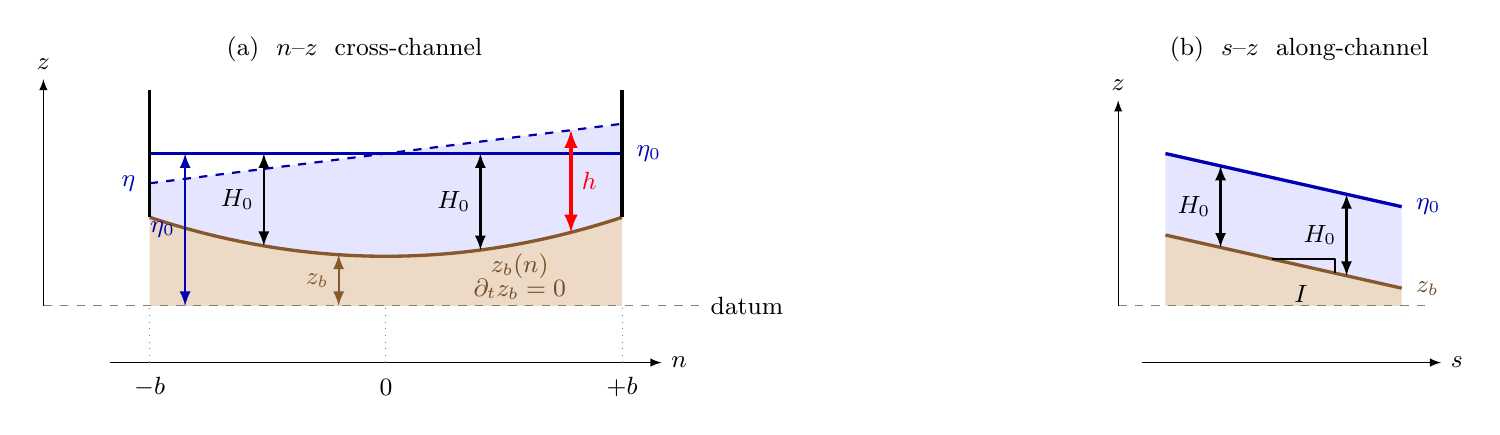
\begin{tikzpicture}[x=1.00cm,y=0.90cm,>=latex,line join=round,font=\small]
% ================= (a) cross-channel =================
  \def\zb(#1){0.70+0.55*(#1/3)^2}      % bed elevation
  \def\eO{2.15}                        % base free surface, flat in n
  \def\eP(#1){2.15+0.42*(#1/3)}        % actual free surface = base + h'
  \fill[blue!10] plot[domain=-3:3,samples=80] (\x,{\zb(\x)})
      -- plot[domain=3:-3,samples=80] (\x,{\eP(\x)}) -- cycle;
  \fill[brown!30] (-3,0) -- (-3,{\zb(-3)})
      -- plot[domain=-3:3,samples=80] (\x,{\zb(\x)}) -- (3,0) -- cycle;
  \draw[brown!70!black,very thick] plot[domain=-3:3,samples=80] (\x,{\zb(\x)});
  \draw[blue!70!black,very thick]  (-3,\eO) -- (3,\eO);
  \draw[blue!70!black,thick,dashed] plot[domain=-3:3,samples=40] (\x,{\eP(\x)});
  \node[blue!70!black,right] at (3.06,\eO) {$\eta_0$};
  \node[blue!70!black,left]  at (-3.06,{\eP(-3)}) {$\eta$};
  \draw[very thick] (-3,{\zb(-3)}) -- (-3,3.05);
  \draw[very thick] ( 3,{\zb(3)})  -- ( 3,3.05);
  \draw[dashed,gray] (-4.35,0) -- (4.00,0) node[right,black]{datum};
  \draw[->] (-4.35,0) -- (-4.35,3.20) node[above]{$z$};
  \draw[->] (-3.5,-0.80) -- (3.5,-0.80) node[right]{$n$};
  \foreach \p/\l in {-3/{-b},0/{0},3/{+b}}{
      \draw[gray,dotted] (\p,-0.80) -- (\p,0);
      \node at (\p,-1.15) {$\l$};}
  % elevations, measured from the datum
  \draw[<->,thick,blue!70!black] (-2.55,0) -- (-2.55,\eO) node[midway,left]{$\eta_0$};
  \draw[<->,thick,brown!70!black] (-0.60,0) -- (-0.60,{\zb(-0.60)})
        node[midway,left]{$z_b$};
  % depths, the gaps
  \draw[<->,thick] (-1.55,{\zb(-1.55)}) -- (-1.55,\eO) node[midway,left]{$H_0$};
  \draw[<->,thick] ( 1.20,{\zb( 1.20)}) -- ( 1.20,\eO) node[midway,left]{$H_0$};
  \draw[<->,very thick,red] (2.35,{\zb(2.35)}) -- (2.35,{\eP(2.35)})
        node[midway,right,red]{$h$};
  \node[brown!60!black] at (1.70,0.56) {$z_b(n)$};
  \node[brown!60!black] at (1.70,0.24) {$\partial_t z_b=0$};
  \node at (-0.4,3.62) {(a)\ \ $n$--$z$\ \ cross-channel};
% ================= (b) along-channel =================
\begin{scope}[xshift=9.9cm]
  \def\zbL(#1){1.00-0.25*#1}
  \def\etL(#1){2.15-0.25*#1}
  \fill[blue!10] (0,{\zbL(0)}) -- (3,{\zbL(3)}) -- (3,{\etL(3)}) -- (0,{\etL(0)}) -- cycle;
  \fill[brown!30] (0,0) -- (3,0) -- (3,{\zbL(3)}) -- (0,{\zbL(0)}) -- cycle;
  \draw[blue!70!black,very thick]  (0,{\etL(0)}) -- (3,{\etL(3)});
  \draw[brown!70!black,very thick] (0,{\zbL(0)}) -- (3,{\zbL(3)});
  \node[blue!70!black,right]  at (3.06,{\etL(3)}) {$\eta_0$};
  \node[brown!60!black,right] at (3.06,{\zbL(3)}) {$z_b$};
  \draw[dashed,gray] (-0.60,0) -- (3.4,0);
  \draw[->] (-0.60,0) -- (-0.60,2.90) node[above]{$z$};
  \draw[->] (-0.30,-0.80) -- (3.5,-0.80) node[right]{$s$};
  \draw[<->,thick] (0.70,{\zbL(0.70)}) -- (0.70,{\etL(0.70)}) node[midway,left]{$H_0$};
  \draw[<->,thick] (2.30,{\zbL(2.30)}) -- (2.30,{\etL(2.30)}) node[midway,left]{$H_0$};
  \draw[thick] (1.35,{\zbL(1.35)}) -- (2.15,{\zbL(1.35)}) -- (2.15,{\zbL(2.15)});
  \node at (1.72,{\zbL(2.15)-0.30}) {$I$};
  \node at (1.70,3.62) {(b)\ \ $s$--$z$\ \ along-channel};
\end{scope}
\end{tikzpicture}
\captionsetup{labelfont={color=red},textfont={color=red}}
\caption{\R{Elevations are measured from the datum; depths are the gaps between
them. $\eta_0$ = base free-surface elevation, $z_b$ = bed elevation,
$H_0=\eta_0-z_b$ = base depth, $h=\eta-z_b=H_0+h'$ = actual depth.
(a) The bed is non-flat in $n$; (10) makes $\eta_0$ flat across the section, so
$H_0(n)=H_0\tilde\xi(\tilde n)^2$ varies with $n$ through the bed alone. The
dashed surface $\eta=\eta_0+h'$ is the perturbation; the gap between the two blue
lines is $h'$. (b) $z_b$ and $\eta_0$ drop together at the valley slope
$I=-\partial_s z_b$, and $-g\partial_s(h+z_b)=-g\partial_s\eta=gI$ drives the
flow. Note $\partial_s z_b\ne0$ --- the bed elevation must fall downstream ---
while $H_0$ and the cross-sectional shape are the same at every $s$. ``The bed
does not change'' means $\partial_t z_b=0$, not $\partial_s z_b=0$.}}
\end{figure}

\R{On the fast time $T_f=\Lambda/U_0$ the flow equilibrates to the (fixed) banks,
so we treat it as \emph{steady}, $\partial_t\to0$; the slow bank motion is restored
in §2.} We non-dimensionalize the
$\mathcal{O}(\varepsilon)$ equation with
\begin{equation}
\tilde u=u'/U,\ \tilde v=v'/V,\ \tilde s=s/\Lambda,\ \tilde n=n/b,\
C'=\mathcal{C}\tilde C(s),\ \tilde h=h'/\mathcal{H}\R{,\ \Lambda=\lambda/2\pi},
\end{equation}
we have
\begin{equation}
\frac{UU_0}{\Lambda}\tilde\xi\dt_s\tilde u
 + \frac{VU_0}{b}\tilde v\dt_n\tilde\xi
= -\frac{g\mathcal{H}}{\Lambda}\dt_s\tilde h
  - \frac{2C_fU_0U}{H_0}\,\R{\frac{\tilde u}{\tilde\xi}}
  + \frac{C_fU_0^2\mathcal{H}}{H_0^2}\,\R{\frac{\tilde h}{\tilde\xi^2}},
\end{equation}
\begin{equation}
\frac{VU_0}{\Lambda}\tilde\xi\dt_s\tilde v
 - \mathcal{C}U_0^2\tilde C\tilde\xi^2
= \G{-\frac{g\mathcal{H}}{b}\dt_n\tilde h}
  - \frac{C_fU_0V}{H_0}\,\R{\frac{\tilde v}{\tilde\xi}},
\end{equation}
\begin{equation}
\frac{\mathcal{H}U_0}{\Lambda}\tilde\xi\dt_s\tilde h
 + \frac{H_0U}{\Lambda}\dt_s\R{(\tilde\xi^2\tilde u)}
 + \frac{H_0V}{b}\dt_n\R{(\tilde\xi^2\tilde v)} = 0 .
\end{equation}
Define
\begin{equation}
\alpha=b/\Lambda,\ \gamma=V/U,\ \varepsilon_1=U/U_0,\
\varepsilon_2=\mathcal{H}/H_0,\ Fr=U_0/\sqrt{gH_0},\
F_c=C_f\Lambda/H_0,\ Ci=\mathcal{C}b
\end{equation}
we have
\begin{equation}
\tilde\xi\dt_s\tilde u
 + \frac{\gamma}{\alpha}\tilde v\dt_n\tilde\xi
= -\frac{\varepsilon_2}{\varepsilon_1Fr^2}\dt_s\tilde h
  - 2F_c\R{\frac{\tilde u}{\tilde\xi}}
  + F_c\frac{\varepsilon_2}{\varepsilon_1}\R{\frac{\tilde h}{\tilde\xi^2}},
\end{equation}
\begin{equation}
\tilde\xi\dt_s\tilde v
 - \frac{Ci}{\varepsilon_1\alpha\gamma}\tilde C\tilde\xi^2
= \G{-\frac{\varepsilon_2}{\varepsilon_1Fr^2\alpha\gamma}\dt_n\tilde h}
  - F_c\R{\frac{\tilde v}{\tilde\xi}},
\end{equation}
\begin{equation}
\dt_s\R{(\tilde\xi^2\tilde u)}
 + \frac{\gamma}{\alpha}\dt_n\R{(\tilde\xi^2\tilde v)}
 + \frac{\varepsilon_2}{\varepsilon_1}
   \R{\tilde\xi\dt_s\tilde h} = 0 .
\end{equation}
\G{\small The green term is the cross-channel superelevation pressure: the free
surface tilts across the channel to balance the centrifugal forcing
$\propto Ci\,\tilde C$, and its streamwise gradient sets the near-bank $u'_b$
(Ikeda's $-U_0^2\partial_s\mathcal{C}'$). Its coefficient
$\varepsilon_2/(\varepsilon_1Fr^2\alpha\gamma)\sim1/(Fr^2\alpha^2)$ is $\ge1$ for
every subcritical ($Fr<1$), long-wave ($\alpha<1$) meander --- $O(1/\varepsilon)$
in limit~1, $O(1)$ in limit~2 --- so it can never be small. That is why limit~2
(the QGPV limit, which \emph{keeps} it) still migrates downstream. Discarding the
free surface entirely (rigid lid, no $\tilde h$) is the only way to remove it;
the pure-vorticity model that then remains migrates upstream on its own
$\beta$-Rossby dynamics.}

We typically assume $\alpha=\gamma$. If we assume
$Ci\sim\varepsilon_1\sim\varepsilon_2\sim\mathcal{O}(\varepsilon)$,
$\alpha\sim\mathcal{O}(\varepsilon^{1/2})$, $Fr\sim F_c\sim1$,
the leading order equation becomes
\begin{equation}
\tilde\xi\dt_s\tilde u+\tilde v\dt_n\tilde\xi
= -\frac{\varepsilon_2}{\varepsilon_1Fr^2}\dt_s\tilde h
  - 2F_c\R{\frac{\tilde u}{\tilde\xi}}
  + F_c\frac{\varepsilon_2}{\varepsilon_1}\R{\frac{\tilde h}{\tilde\xi^2}},
\end{equation}
\begin{equation}
\frac{1}{\varepsilon_1\alpha^2}Ci\,\tilde C\tilde\xi^2
= \G{\frac{1}{\varepsilon_1\alpha^2}\frac{\varepsilon_2}{Fr^2}\dt_n\tilde h},
\end{equation}
\begin{equation}
\dt_s\R{(\tilde\xi^2\tilde u)}+\dt_n\R{(\tilde\xi^2\tilde v)}
 + \frac{\varepsilon_2}{\varepsilon_1}
   \R{\tilde\xi\dt_s\tilde h} = 0 .
\end{equation}
Equations 20 and Equation 21 lead to the solution in Ikeda et al.

If we assume that $\varepsilon_2\sim\mathcal{O}(\varepsilon^2)$,
$Ci\sim\varepsilon_1\sim Fr^2\sim\mathcal{O}(\varepsilon)$, and set $\alpha=1$
\R{(so $Ci/\varepsilon_1=O(1)$: the curvature forcing survives --- a
\emph{forced} QGPV, as in §1.1)}, the leading order equation becomes
\begin{equation}
\tilde\xi\dt_s\tilde u+\tilde v\dt_n\tilde\xi
= -\frac{\varepsilon_2}{\varepsilon_1Fr^2}\dt_s\tilde h
  - 2F_c\R{\frac{\tilde u}{\tilde\xi}},
\end{equation}
\begin{equation}
\tilde\xi\dt_s\tilde v
 - \R{\frac{Ci}{\varepsilon_1\alpha^2}\tilde C\tilde\xi^2}
= \G{-\frac{\varepsilon_2}{\varepsilon_1Fr^2}\dt_n\tilde h}
  - F_c\R{\frac{\tilde v}{\tilde\xi}},
\end{equation}
\begin{equation}
\dt_s\R{(\tilde\xi^2\tilde u)}+\dt_n\R{(\tilde\xi^2\tilde v)} = 0 .
\end{equation}
Equations 23-25 leads to the QGPV equation
\begin{equation}
\tilde\xi\dt_s\R{\tilde\zeta}+\tilde\beta\tilde v
= \R{-\frac{F_c}{\tilde\xi}\tilde\zeta
    + \frac{F_c}{\tilde\xi}\dt_n\tilde u
    - \frac{2F_c\tilde u}{\tilde\xi^{2}}\dt_n\tilde\xi
    + \frac{Ci}{\varepsilon_1\alpha^2}\tilde\xi^2\dt_s\tilde C},
\end{equation}
where
\begin{equation}
\tilde\beta=\R{2\frac{(\dt_n\tilde\xi)^2}{\tilde\xi}}-\dt_{nn}\tilde\xi,\qquad
\R{\tilde\zeta}=\dt_s\tilde v-\dt_n\tilde u,\qquad
\R{\tilde\xi^2\tilde u=-\dt_n\tilde\psi,\quad
   \tilde\xi^2\tilde v=\dt_s\tilde\psi .}
\end{equation}
\R{With the \emph{flat-bed} choice $H_0=\mathrm{const}$ (rather than the balanced
$H_0=H_0\tilde\xi^2$ derived at (9)--(11)), the friction denominators lose a
power of $\tilde\xi$ ($\tilde u/\tilde\xi\to\tilde\xi\,\tilde u$), continuity (25)
becomes the non-divergent $\dt_s\tilde u+\dt_n\tilde v=0$, and
$\tilde\beta\to-\dt_{nn}\tilde\xi$; equations (23)--(27) then coincide
term-for-term with the July-24 update. The slaved-bed form above ($H_0=\tilde\xi^2$)
is the self-consistent one --- its base state actually exists --- and is what the
Thetis model solves.}

We can put:
\begin{equation}
\tilde\xi(\tilde n)\dt_s\tilde u
 + \tilde v\dt_n\tilde\xi(\tilde n)
 + \frac{\varepsilon_2}{\varepsilon_1Fr^2}\dt_s\tilde h
 + 2F_c\R{\frac{\tilde u}{\tilde\xi(\tilde n)}}
 - F_c\frac{\varepsilon_2}{\varepsilon_1}
   \R{\frac{\tilde h}{\tilde\xi(\tilde n)^2}} = 0,
\end{equation}
\begin{equation}
\tilde\xi(\tilde n)\dt_s\tilde v
 - \frac{Ci}{\varepsilon_1\alpha^2}\tilde C(\tilde s)\tilde\xi(\tilde n)^2
 + \G{\frac{\varepsilon_2}{\varepsilon_1Fr^2\alpha^2}\dt_n\tilde h}
 + F_c\R{\frac{\tilde v}{\tilde\xi(\tilde n)}} = 0,
\end{equation}
\begin{equation}
\dt_s\R{\bigl(\tilde\xi(\tilde n)^2\tilde u\bigr)}
 + \dt_n\R{\bigl(\tilde\xi(\tilde n)^2\tilde v\bigr)}
 + \frac{\varepsilon_2}{\varepsilon_1}
   \R{\tilde\xi(\tilde n)\dt_s\tilde h} = 0 .
\end{equation}

\R{\subsection*{From gravity to Rossby: the curl and its ordering}}

\R{Equations (17)--(19) carry seven groups $\alpha,\gamma,\varepsilon_1,
\varepsilon_2,Fr,F_c,Ci$ (with $\alpha=\gamma$); their relative orders decide
whether the leading balance is the gravity/Ikeda response or a Rossby wave. The
Rossby branch lives on the \emph{vorticity} equation, obtained by the curl
$\dt_s(18)-\dt_n(17)$. Write $P_s=\varepsilon_2/(\varepsilon_1Fr^2)$ (the
$\dt_s\tilde h$ coefficient in (17)) and
$P_n=\varepsilon_2/(\varepsilon_1Fr^2\alpha\gamma)=P_s/(\alpha\gamma)$ (the
$\dt_n\tilde h$ coefficient in (18)); the two pressure terms combine as}
\begin{equation*}
\R{\dt_s\!\big(P_n\dt_n\tilde h\big)-\dt_n\!\big(P_s\dt_s\tilde h\big)
 =(P_n-P_s)\,\dt_s\dt_n\tilde h
 =P_s\Big(\tfrac{1}{\alpha\gamma}-1\Big)\dt_s\dt_n\tilde h ,}
\end{equation*}
\R{which vanishes \emph{identically} iff $P_n=P_s$, i.e.\ $\boxed{\alpha\gamma=1}$,
hence $\alpha=\gamma=1$: the pressure cancels in the curl. This is geometric and
$Fr$-independent, and it is a \emph{coefficient match}, not a smallness --- with
$Fr^2\sim\varepsilon_1$ the pressure $P_s=O(1)$ is a leading-order term of the
un-curled momentum equations; it leaves the \emph{vorticity} budget only because
$\alpha=1$ equalises the two length scales $\Lambda,b$. When $\alpha\ll1$ (Ikeda)
$P_n=P_s/\alpha^2\gg P_s$: the $\dt_n\tilde h$ pressure dominates (18) ---
cross-channel superelevation, a gravity response with no vorticity dynamics.}

\R{With $\alpha=\gamma=1$, continuity (19) is non-divergent provided
$\varepsilon_2/\varepsilon_1\ll1$ (rigid lid), so a streamfunction exists
($\tilde\xi^2\tilde u=-\dt_n\tilde\psi,\ \tilde\xi^2\tilde v=\dt_s\tilde\psi$) and
$\dt_s\tilde u+\dt_n\tilde v=-2(\dt_n\tilde\xi/\tilde\xi)\tilde v$. Substituting
into the curled inertia gives the jet's background PV gradient}
\begin{equation*}
\R{\tilde\beta=\frac{2(\dt_n\tilde\xi)^2}{\tilde\xi}-\dt_{nn}\tilde\xi
 =\tilde\xi^2\,\dt_n q_{\mathrm{base}},\qquad
 q_{\mathrm{base}}=-\frac{\dt_n\tilde\xi}{\tilde\xi^2}}
\end{equation*}
\R{(base velocity $\tilde\xi$, base depth $\tilde\xi^2$). The
$+2(\dt_n\tilde\xi)^2/\tilde\xi$ term is the depth-slaving signature --- a
constant-depth base drops it and leaves the wrong $-\dt_{nn}\tilde\xi$; a uniform
jet has $\tilde\beta=0$ and no wave. The leading-order vorticity equation is}
\begin{equation*}
\R{\tilde\xi\,\dt_s\tilde\zeta+\tilde\beta\,\tilde v
 +\frac{F_c}{\tilde\xi}\big[\tilde\zeta-\tilde\xi^2\dt_n(\tilde u/\tilde\xi^2)\big]
 =\frac{Ci}{\varepsilon_1}\,\tilde\xi^2\,\dt_s\tilde C ,\quad
 \tilde\zeta=\dt_s\tilde v-\dt_n\tilde u }\tag{$\star$}
\end{equation*}
\R{--- advection of vorticity along the jet, the shear-Rossby restoring
$\tilde\beta\tilde v$, quadratic bottom-drag (the factor-2 asymmetry
$2F_c\tilde u/\tilde\xi$ vs $F_c\tilde v/\tilde\xi$), and the curvature forcing;
exactly the $U q'_x+v'Q_y=\text{friction}$ form.}

\R{The orderings that select each branch:}
\begin{center}\small\color{red}
\begin{tabular}{lccc}
parameter & Rossby / QGPV & Gravity / Ikeda & role\\
\hline
$\alpha=\gamma$ & $O(1)\ [{=}1]$ & $O(\varepsilon^{1/2})$ & pressure cancels vs dominates\\
$\varepsilon_2/\varepsilon_1$ & $O(\varepsilon)$ & $O(1)$ & (non-)divergent\\
$Fr^2$ & $O(\varepsilon)$ & $O(1)$ & low- vs finite-Froude\\
$Ci/\varepsilon_1$ & $O(1)$ forced & $O(1)$ & curvature source\\
$F_c$ & $O(1)$ & $O(1)$ & friction leading order\\
\end{tabular}
\end{center}
\R{The single switch is $\alpha\gamma$: $=1$ Rossby (pressure curls away), $\ll1$
gravity (pressure dominates (18)); low $Fr$ is the consistent secondary marker.
Forced vs free is $Ci/\varepsilon_1$ ($O(1)$ keeps the source through
$\dt_s\tilde C$; $\ll1$ leaves the free shear-Rossby wave).}

\R{\section{Slow timescale: bank migration}}

\R{Section 1's flow is steady on the fast time $T_f=\Lambda/U_0$: given the banks
it equilibrates within a few advection times. The banks themselves move on a much
slower time set by the erosion law. Let $y_b(s,t)$ be a bank's lateral position
and $u_b'=u'(s,\pm b)$ the near-bank velocity from §1; with
$\psi_1',\psi_2',\psi_3'$ the streamfunction perturbation at $n=+b,\,0,\,-b$,}
\begin{equation}
\R{\psi_1'=\bar u(b)\,y_b=U_0\,y_b ,}
\end{equation}
\begin{equation}
\R{u_b'=\bigl(\psi_2'-\psi_1'\bigr)/b ,}
\end{equation}
\begin{equation}
\R{\partial_t\psi_1'=\frac{\varepsilon C_fU_0}{b}\bigl(\psi_2'-\psi_1'\bigr) ,}
\end{equation}
\begin{equation}
\R{\gamma\,\partial_t y_b=E\,u_b' ,\qquad E=\varepsilon C_f ,\qquad
\gamma=\cos\theta .}
\end{equation}
\R{Equation (33) is the three-level form; (34) is Ikeda, Parker \& Sawai
(1981) eqs (11)--(13). For two independently mobile banks $y_N,y_S$,}
\begin{equation}
\R{\partial_t y_N=+E_{e,d}\,u_N' ,\qquad
   \partial_t y_S=-E_{e,d}\,u_S' ,}
\end{equation}
\R{with $E_e$ where $u'>0$ (erosion) and $E_d$ where $u'<0$ (deposition);
$E_e=E_d$ gives constant width.}

\R{\paragraph{The slow timescale.} How long does a bank take to move? Scale
$y_b\sim b$ and $u_b'\sim U=\varepsilon_1U_0$, and rescale time $t=T_s\tau$ in (34):}
\begin{equation}
\R{\gamma\,\frac{b}{T_s}\,\partial_\tau\tilde y_b=\varepsilon C_f\,U\,\tilde u_b'
 \quad\Longrightarrow\quad
 T_s=\frac{\gamma\,b}{\varepsilon C_f\,U}
    =\frac{\gamma\,b}{\varepsilon C_f\,\varepsilon_1U_0},}
\end{equation}
\R{chosen so the bank evolves at $O(1)$, $\partial_\tau\tilde y_b=\tilde u_b'$.
The flow and the bank are thus non-dimensionalized by \emph{different} time
parameters --- $T_f=\Lambda/U_0$ (advection) and $T_s$ (erosion) --- with ratio}
\begin{equation}
\R{\frac{T_f}{T_s}=\frac{\varepsilon C_f\,\varepsilon_1}{\gamma\,\alpha}\ll1,
 \qquad\alpha=\frac{b}{\Lambda}.}
\end{equation}
\R{This ratio --- the product of the erosion coefficient $\varepsilon C_f$ and the
flow perturbation $\varepsilon_1$, \emph{not} the $\varepsilon$ of §1 --- is the
genuine small parameter of the morphodynamics. Because $T_f/T_s\ll1$, the
$\partial_t$ acting on the flow is negligible: this is precisely why §1 is steady,
the flow adiabatically following the instantaneous planform while all time
evolution lives on the bank. The meander grows and migrates on $T_s$.}

\R{\section{Secondary flow and the bed --- the $A$ switch}}

\R{The note has no secondary-flow term; a depth-averaged 2-D model cannot
generate the helical circulation of a bend, so its effect on the bed is
\emph{imposed} as a curvature-slaved perturbation to the frozen depth of §1.
Writing the total depth as $H(s,n)=H_0(n)+H_2'(s,n)$ with $H_0(n)$ the
time-independent base profile, Ikeda, Parker \& Sawai (1981) eq.~(6) is}
\begin{equation}
\R{H_2'(s,n) = -A\,H_0(n)\,\mathcal{C}'(s)\,n ,\qquad n=b\tilde n ,}
\end{equation}
\R{a pool ($H_2'>0$, deeper) on the outer bank and a point bar on the inner
bank, both proportional to the local centreline curvature $\mathcal{C}'(s)$.
(This is Ikeda's bed perturbation $\eta'$, renamed to avoid clashing with the
free surface $\eta$; the sign is fixed so the pool is on the outer bank. It
enters the bed of §1 as $z_b=\bar z_b(n)+z_b'$ with $z_b'=-H_2'$.)  The
secondary-flow strength is a switch,}
\begin{equation}
\R{A=0:\ \text{incised, no secondary flow}\ (H_2'\equiv0,\ \text{frozen bed});
   \qquad A=2.89:\ \text{alluvial (Suga 1963).}}
\end{equation}
\R{$H_0(n)$ never changes in time; $H_2'$ carries no independent dynamics --- it
is slaved to the slowly migrating planform (recomputed from the current
curvature each morphological step), so ``the bed does not change'' still means
$\partial_t z_b=0$.  With $h'=\xi'-\eta'$ and Ikeda's superelevation
$\xi'=\mathcal{C}'U_0^2 n/g$, the depth perturbation is
$h'/H_0=(F^2+A)\,\mathcal{C}'\tilde n$: $A$ and $F^2$ occupy the \emph{same}
depth/drag slot, so $A=0$ leaves only $F^2\!\approx\!0.09$ while $A=2.89$ raises
the bend forcing to $\approx2.98$ --- which is what turns bend decay into
growth.}

\R{\section{Boundary conditions}}

\R{The note is an interior linear analysis and states no boundary conditions;
the model closes the channel $[0,L]\times[-b,b]$ with}
\begin{equation}
\R{\underbrace{u_n=-\bar u(n)}_{\text{inflow }s=0},\qquad
   \underbrace{\eta=\eta_{\mathrm{ref}}-I\,L}_{\text{outflow }s=L},\qquad
   \underbrace{u_n=0}_{\text{banks }n=\pm b} .}
\end{equation}
\R{The flow is subcritical ($Fr<1$), so exactly one characteristic enters at
each open boundary: the inflow prescribes the velocity profile only, the
outflow the elevation only. Pinning $\eta$, $u$ and $v$ together at one open
boundary would over-determine it (and, started from rest, launch a spurious
bore). The banks are free-slip --- no normal flux, no wall drag beyond the bed
friction. Drag is quadratic, $-C_f|\bu|\bu/h$ with $C_f=0.05$; a small
horizontal viscosity $\nu=0.05\,\mathrm{m^2\,s^{-1}}$ is retained for
DG stability (both stated here because the note carries neither).}

\end{document}
